% !TEX program = xelatex
% What "after the first touch" is: the rule that gives every corner shot its segment (definitions.md §4), written as four
% questions applied in order, each answer sending the shot to its segment. renders/render_segments.py
% writes segments-defs.tex (each segment's name, gloss, shots and goals from the record) and compiles this file from this
% folder with that file on TEXINPUTS; tests/test_drivers_smoke.py checks the definitions against the record.
\documentclass[border=0pt]{standalone}
% The paper's diagrams in TikZ: Hudl's colours and Barlow, the values of src/viz/paper.py, on the light card the charts sit
% on. Font paths are relative to this folder, so compile from it (renders/render_segments.py does).
\usepackage{fontspec}
\usepackage{tikz}
\usetikzlibrary{arrows.meta,calc}
\setmainfont{Barlow}[Path=../../figures/fonts/, Extension=.ttf, UprightFont=*-Regular, BoldFont=*-Bold]
\newfontfamily\medium{Barlow}[Path=../../figures/fonts/, Extension=.ttf, UprightFont=*-Medium]
% a label never breaks a word
\hyphenpenalty=10000 \exhyphenpenalty=10000
\frenchspacing

\definecolor{page}{HTML}{F9FAFB}
\definecolor{ink}{HTML}{232A31}
\definecolor{ink2}{HTML}{4E5D6C}
\definecolor{context}{HTML}{B1BCC4}
\definecolor{after}{HTML}{FF6300}

\pgfdeclarelayer{canvas}
\pgfsetlayers{canvas,main}

% the type sizes of the charts: 7.5 pt for a name, 7 pt for the rest
\newcommand{\hd}{\fontsize{7.5}{9}\selectfont\bfseries}
\newcommand{\bd}{\fontsize{7}{8.4}\selectfont}

\tikzset{
  flow/.style={-{Stealth[length=4pt]}, draw=ink2, line width=0.6pt},
  box/.style={draw=context, line width=0.6pt, fill=white, rounded corners=2pt, inner sep=0pt},
  answer/.style={font=\bd\medium, text=ink2, inner sep=2pt},
}

\input{segments-defs}

% \question{node}{y}{number}{text}: a question of the rule, on the left
\newcommand{\question}[4]{%
  \node[box, minimum width=6.6cm, minimum height=0.8cm, anchor=west] (#1) at (0.3,#2) {};
  \node[anchor=west, font=\hd, text=ink2] at ([xshift=0.25cm]#1.west) {#3};
  \node[anchor=west, font=\bd, text=ink, text width=5.7cm, align=left] at ([xshift=0.6cm]#1.west) {#4};}
% \segment{key}{y}{bar colour}{border style}: a segment on the right, its name and gloss on the left of the box and its
% shots and goals on the right, from the definitions the driver writes
\newcommand{\segment}[4]{%
  \node[box, #4, minimum width=5.2cm, minimum height=0.8cm, anchor=west] (#1) at (8.1,#2) {};
  \ifx&#3&\else\fill[#3] (#1.north west) rectangle ([xshift=0.09cm]#1.south west);\fi
  \node[anchor=west, font=\hd, text=ink] at ([xshift=0.3cm, yshift=0.17cm]#1.west) {\csname #1name\endcsname};
  \node[anchor=west, font=\bd, text=ink2] at ([xshift=0.3cm, yshift=-0.17cm]#1.west) {\csname #1says\endcsname};
  \node[anchor=east, font=\hd, text=ink] at ([xshift=-0.25cm, yshift=0.17cm]#1.east) {\csname #1shots\endcsname\ shots};
  \node[anchor=east, font=\bd, text=ink] at ([xshift=-0.25cm, yshift=-0.17cm]#1.east) {\csname #1goals\endcsname\ goals};}

\begin{document}
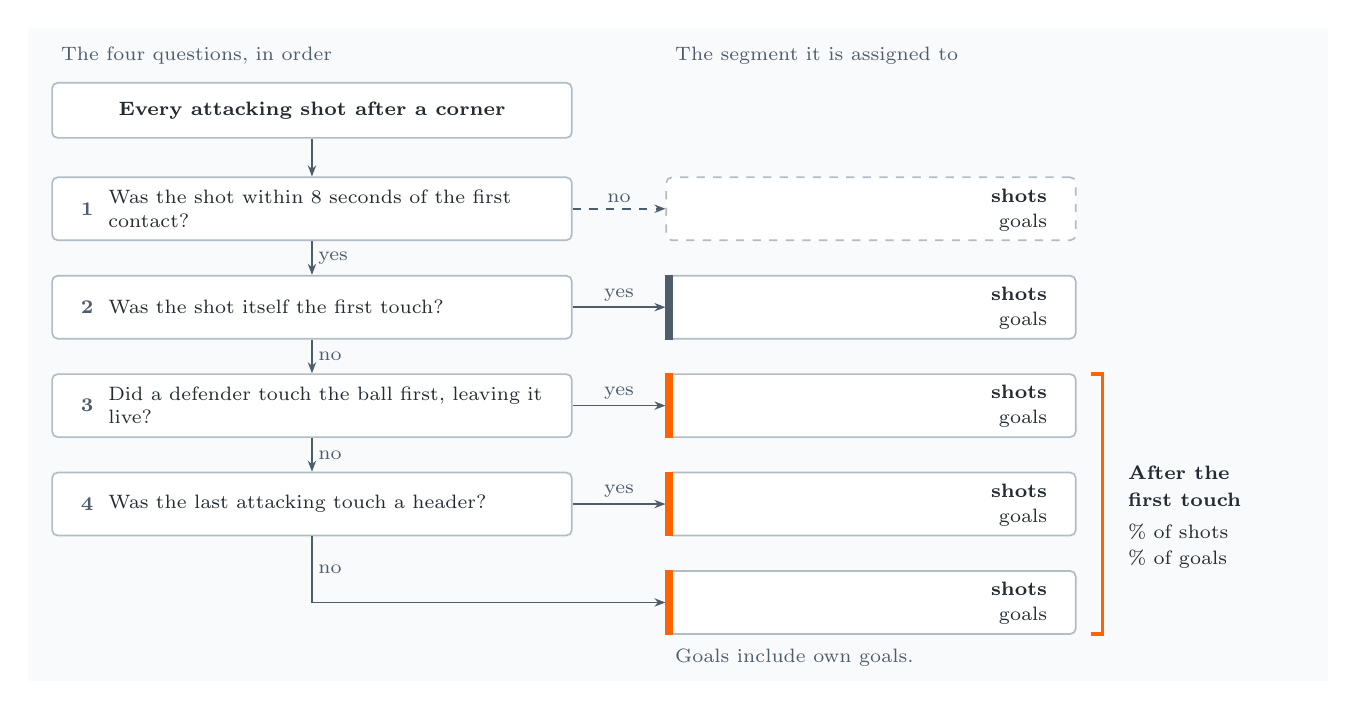
\begin{tikzpicture}
\begin{pgfonlayer}{canvas}\fill[page] (0,0) rectangle (16.51,8.3);\end{pgfonlayer}
\node[anchor=west, font=\bd\medium, text=ink2] at (0.3,7.95) {The four questions, in order};
\node[anchor=west, font=\bd\medium, text=ink2] at (8.1,7.95) {The segment it is assigned to};

\node[box, minimum width=6.6cm, minimum height=0.7cm, anchor=west, font=\hd, text=ink] (root) at (0.3,7.25)
  {Every attacking shot after a corner};
\question{q1}{6.0}{1}{Was the shot within 8 seconds of the first contact?}
\question{q2}{4.75}{2}{Was the shot itself the first touch?}
\question{q3}{3.5}{3}{Did a defender touch the ball first, leaving it live?}
\question{q4}{2.25}{4}{Was the last attacking touch a header?}

\segment{late}{6.0}{}{dashed}
\segment{direct}{4.75}{ink2}{}
\segment{afterclearance}{3.5}{after}{}
\segment{flickon}{2.25}{after}{}
\segment{prolongation}{1.0}{after}{}

\draw[flow] (root.south) -- (q1.north);
\draw[flow] (q1.south) -- node[answer, right] {yes} (q2.north);
\draw[flow] (q2.south) -- node[answer, right] {no} (q3.north);
\draw[flow] (q3.south) -- node[answer, right] {no} (q4.north);
\draw[flow, dashed] (q1.east) -- node[answer, above] {no} (late.west);
\draw[flow] (q2.east) -- node[answer, above] {yes} (direct.west);
\draw[flow] (q3.east) -- node[answer, above] {yes} (afterclearance.west);
\draw[flow] (q4.east) -- node[answer, above] {yes} (flickon.west);
\draw[flow] (q4.south) |- node[answer, right, pos=0.25] {no} (prolongation.west);

% the three segments after the first touch, and their share of the shots and goals
\draw[after, line width=1.2pt] (13.5,3.9) -- (13.65,3.9) -- (13.65,0.6) -- (13.5,0.6);
\node[anchor=west, font=\bd, text=ink2] at (8.1,0.3) {Goals include own goals.};
\node[anchor=west, font=\hd, text=ink] at (13.85,2.65) {After the};
\node[anchor=west, font=\hd, text=ink] at (13.85,2.3) {first touch};
\node[anchor=west, font=\bd, text=ink] at (13.85,1.9) {\aftshots\% of shots};
\node[anchor=west, font=\bd, text=ink] at (13.85,1.55) {\aftgoals\% of goals};
\end{tikzpicture}
\end{document}
